\documentclass[12pt,a4paper]{article}
% The following LaTeX packages must be installed on your machine: amsmath, authblk, bm, booktabs, caption, dcolumn, fancyhdr, geometry, graphicx, hyperref, latexsym, natbib
\input{183.dat}
\usepackage{gensymb}
\usepackage{amsthm}
\usepackage{float}
\usepackage{siunitx}
\usepackage{amssymb}
\usepackage{float}
\usepackage{enumerate}
\usepackage{listings}
\usepackage{mathtools}
\PassOptionsToPackage{hyphens}{url}\usepackage{hyperref}
\usepackage[none]{hyphenat}
\usepackage{physics}
\newcommand\ddfrac[2]{\frac{\displaystyle #1}{\displaystyle #2}}
%\renewcommand{\familydefault}{\sfdefault}


\begin{document}

\setcounter{page}{1}

\section*{Describing Functions}
\bigskip

\begin{enumerate}[1.]

\item \textbf{Saturation/Limiter}

\begin{figure}[h!]
	\centering
	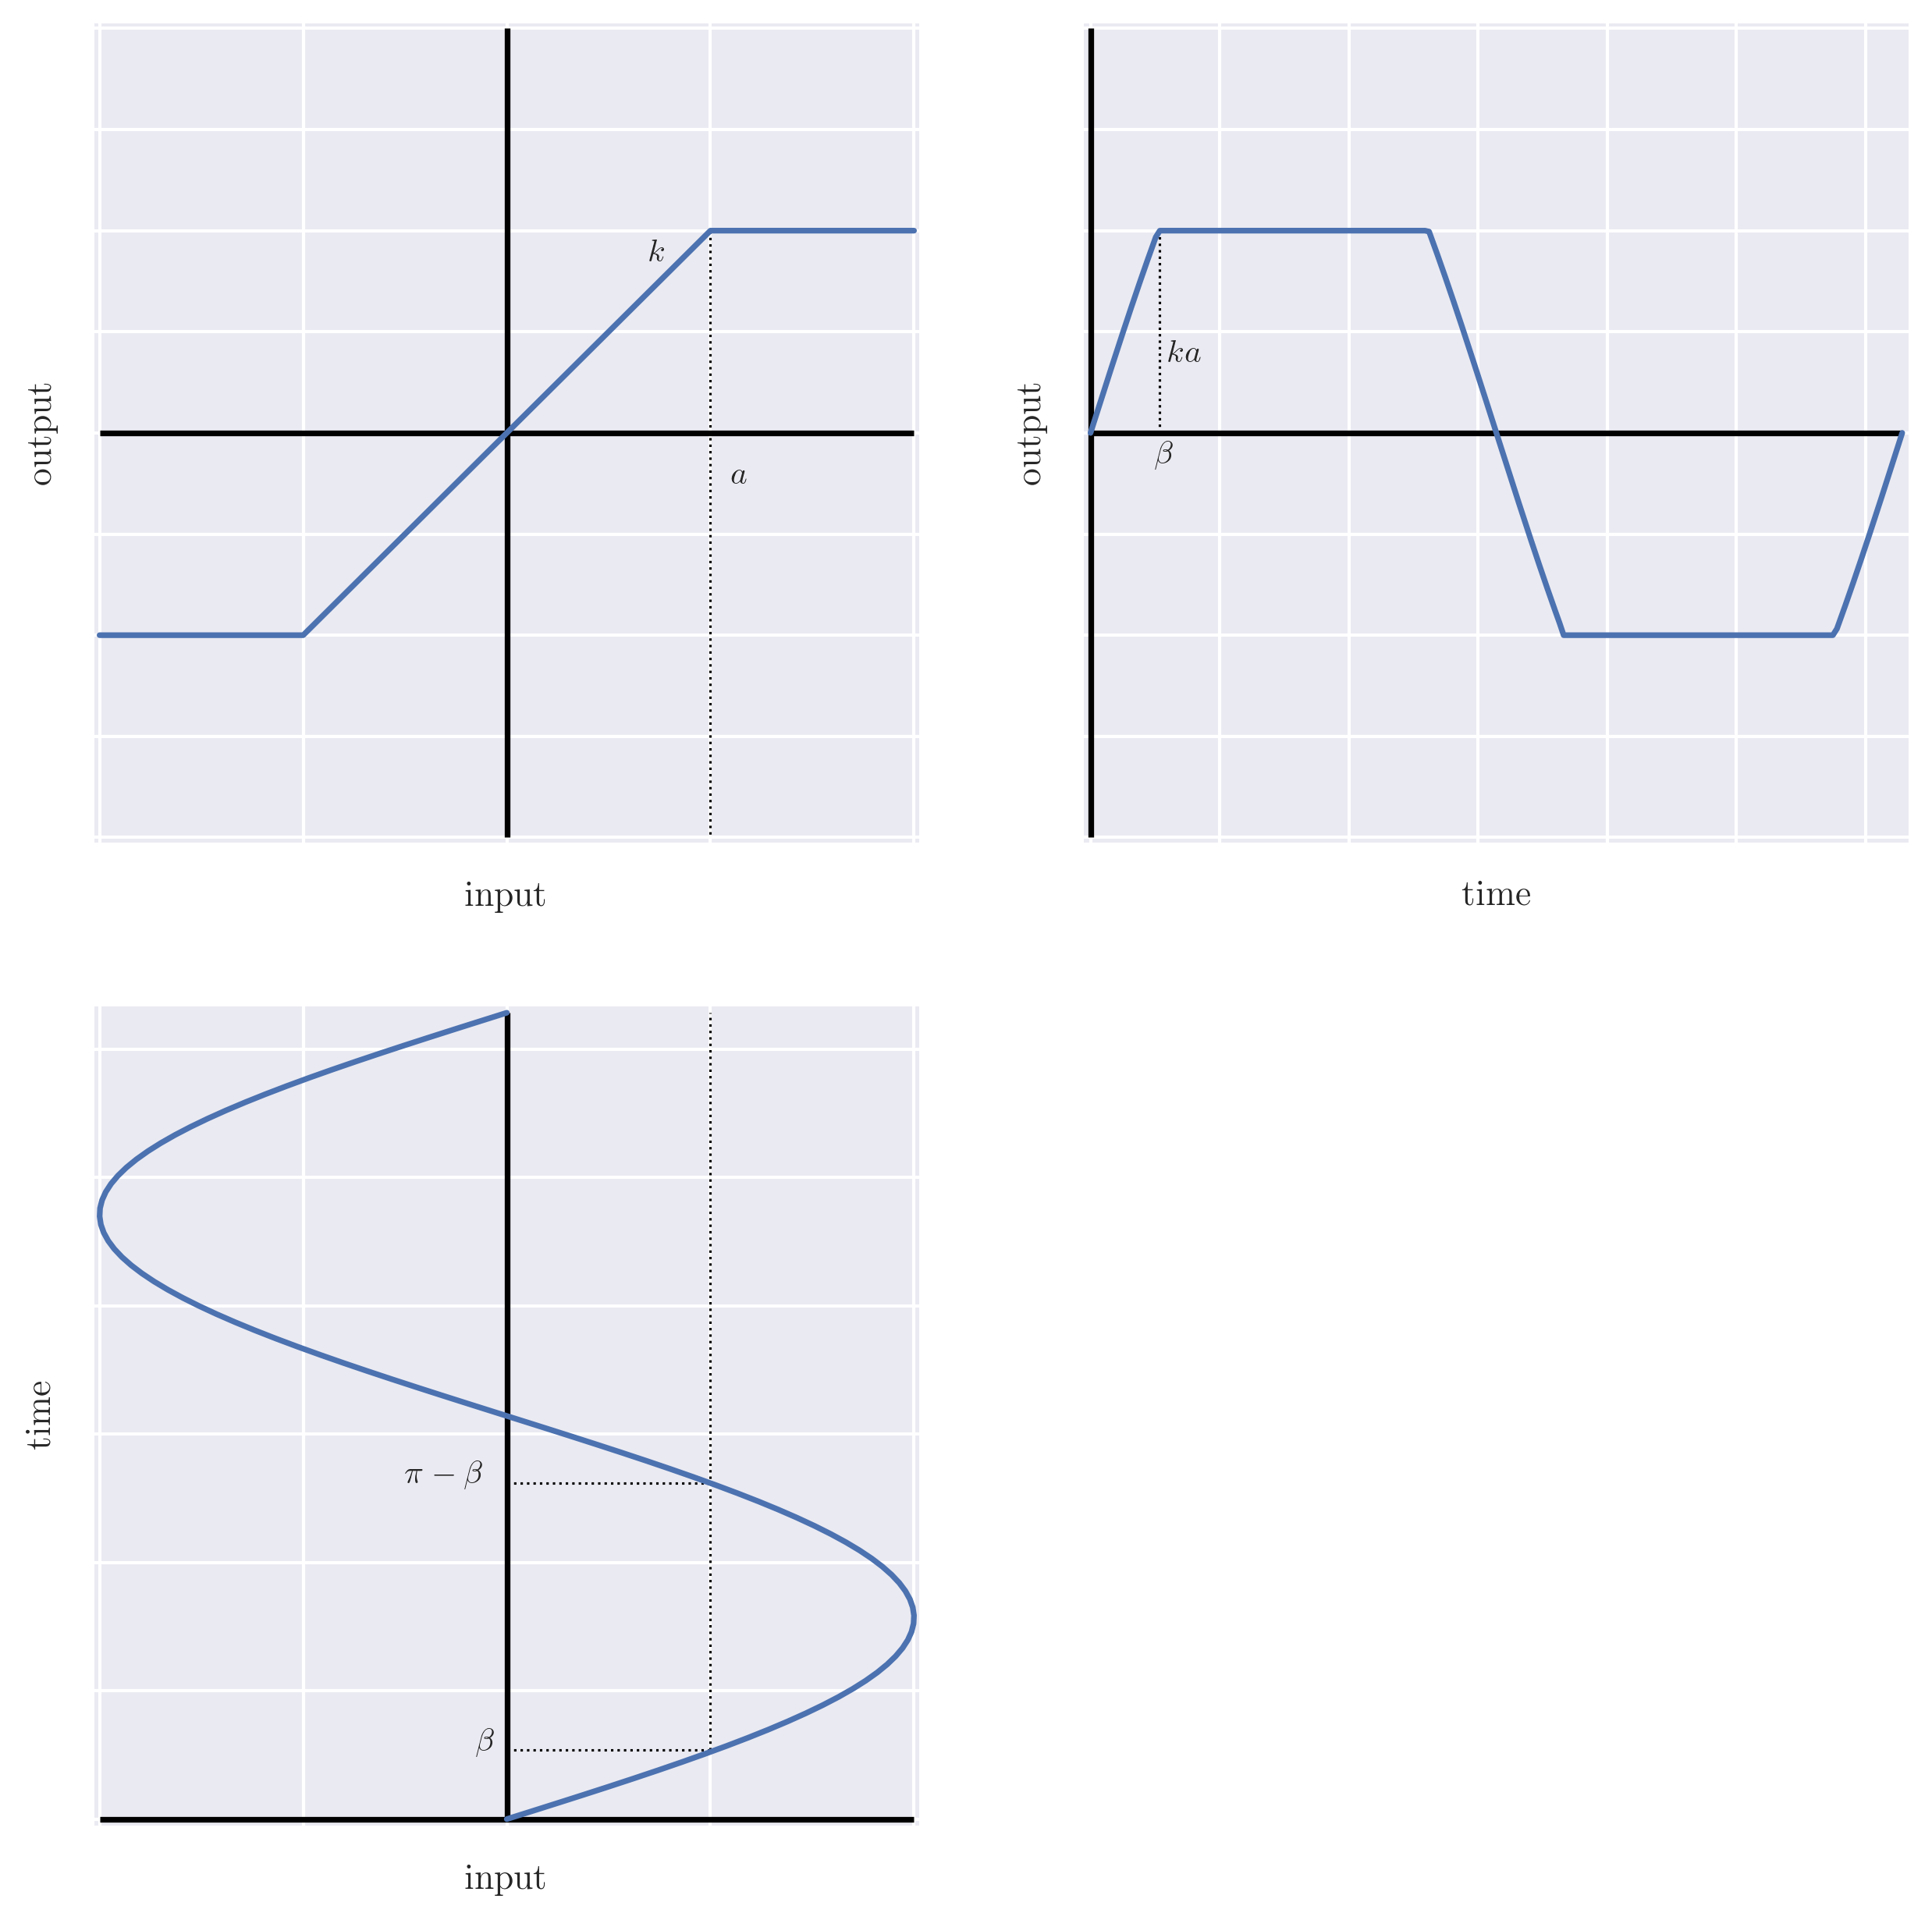
\includegraphics[width=\linewidth]{iocurve.png}
	\caption{IO curves of a saturation function with a sinusoidal input.}
	\label{fig:iocurve}
\end{figure}

Consider an input of the form $V\sin(\omega t)$. The output function is described as 

\begin{equation}
  n(t) =
  \begin{cases}
  	kV\sin(\omega t) & , \quad 0 \leq \omega t \leq \beta \\
  	ka & , \quad \beta \leq \omega t \leq (\pi - \beta) \\
  	kV\sin(\omega t) & , \quad (\pi - \beta) \leq \omega t \leq \pi
  \end{cases}
\end{equation}

We cascade this nonlinear system with a some linear system $G(s)$, typically a low-pass filter and equate it to the first terms of the Fourier series:

\begin{equation}
	n(t) = A_1 \cos(\omega t) + B_1 \sin(\omega t)
\end{equation}

Let $T \equiv 2\pi/\omega$ and calculate the coefficients $A_1$ and $B_1$:

\begin{align}
	A_1 &= \frac{2}{T} \int_{t_0}^{t_0 + T} n(t)\cos(\omega t) \dd{t} \\
	B_1 &= \frac{2}{T} \int_{t_0}^{t_0 + T} n(t)\sin(\omega t) \dd{t}
\end{align}

We evaluate the integral over one full period from initial time $t_0$. For simplicity, we let $t_0 = 0$. Graphically, to get $A_1$, we multiply $n(t)$ with $\cos(\omega t)$ then get the area under the curve over one full period, as shown in Fig. \ref{fig:prod-ncos}.

\begin{figure}[h!]
	\centering
	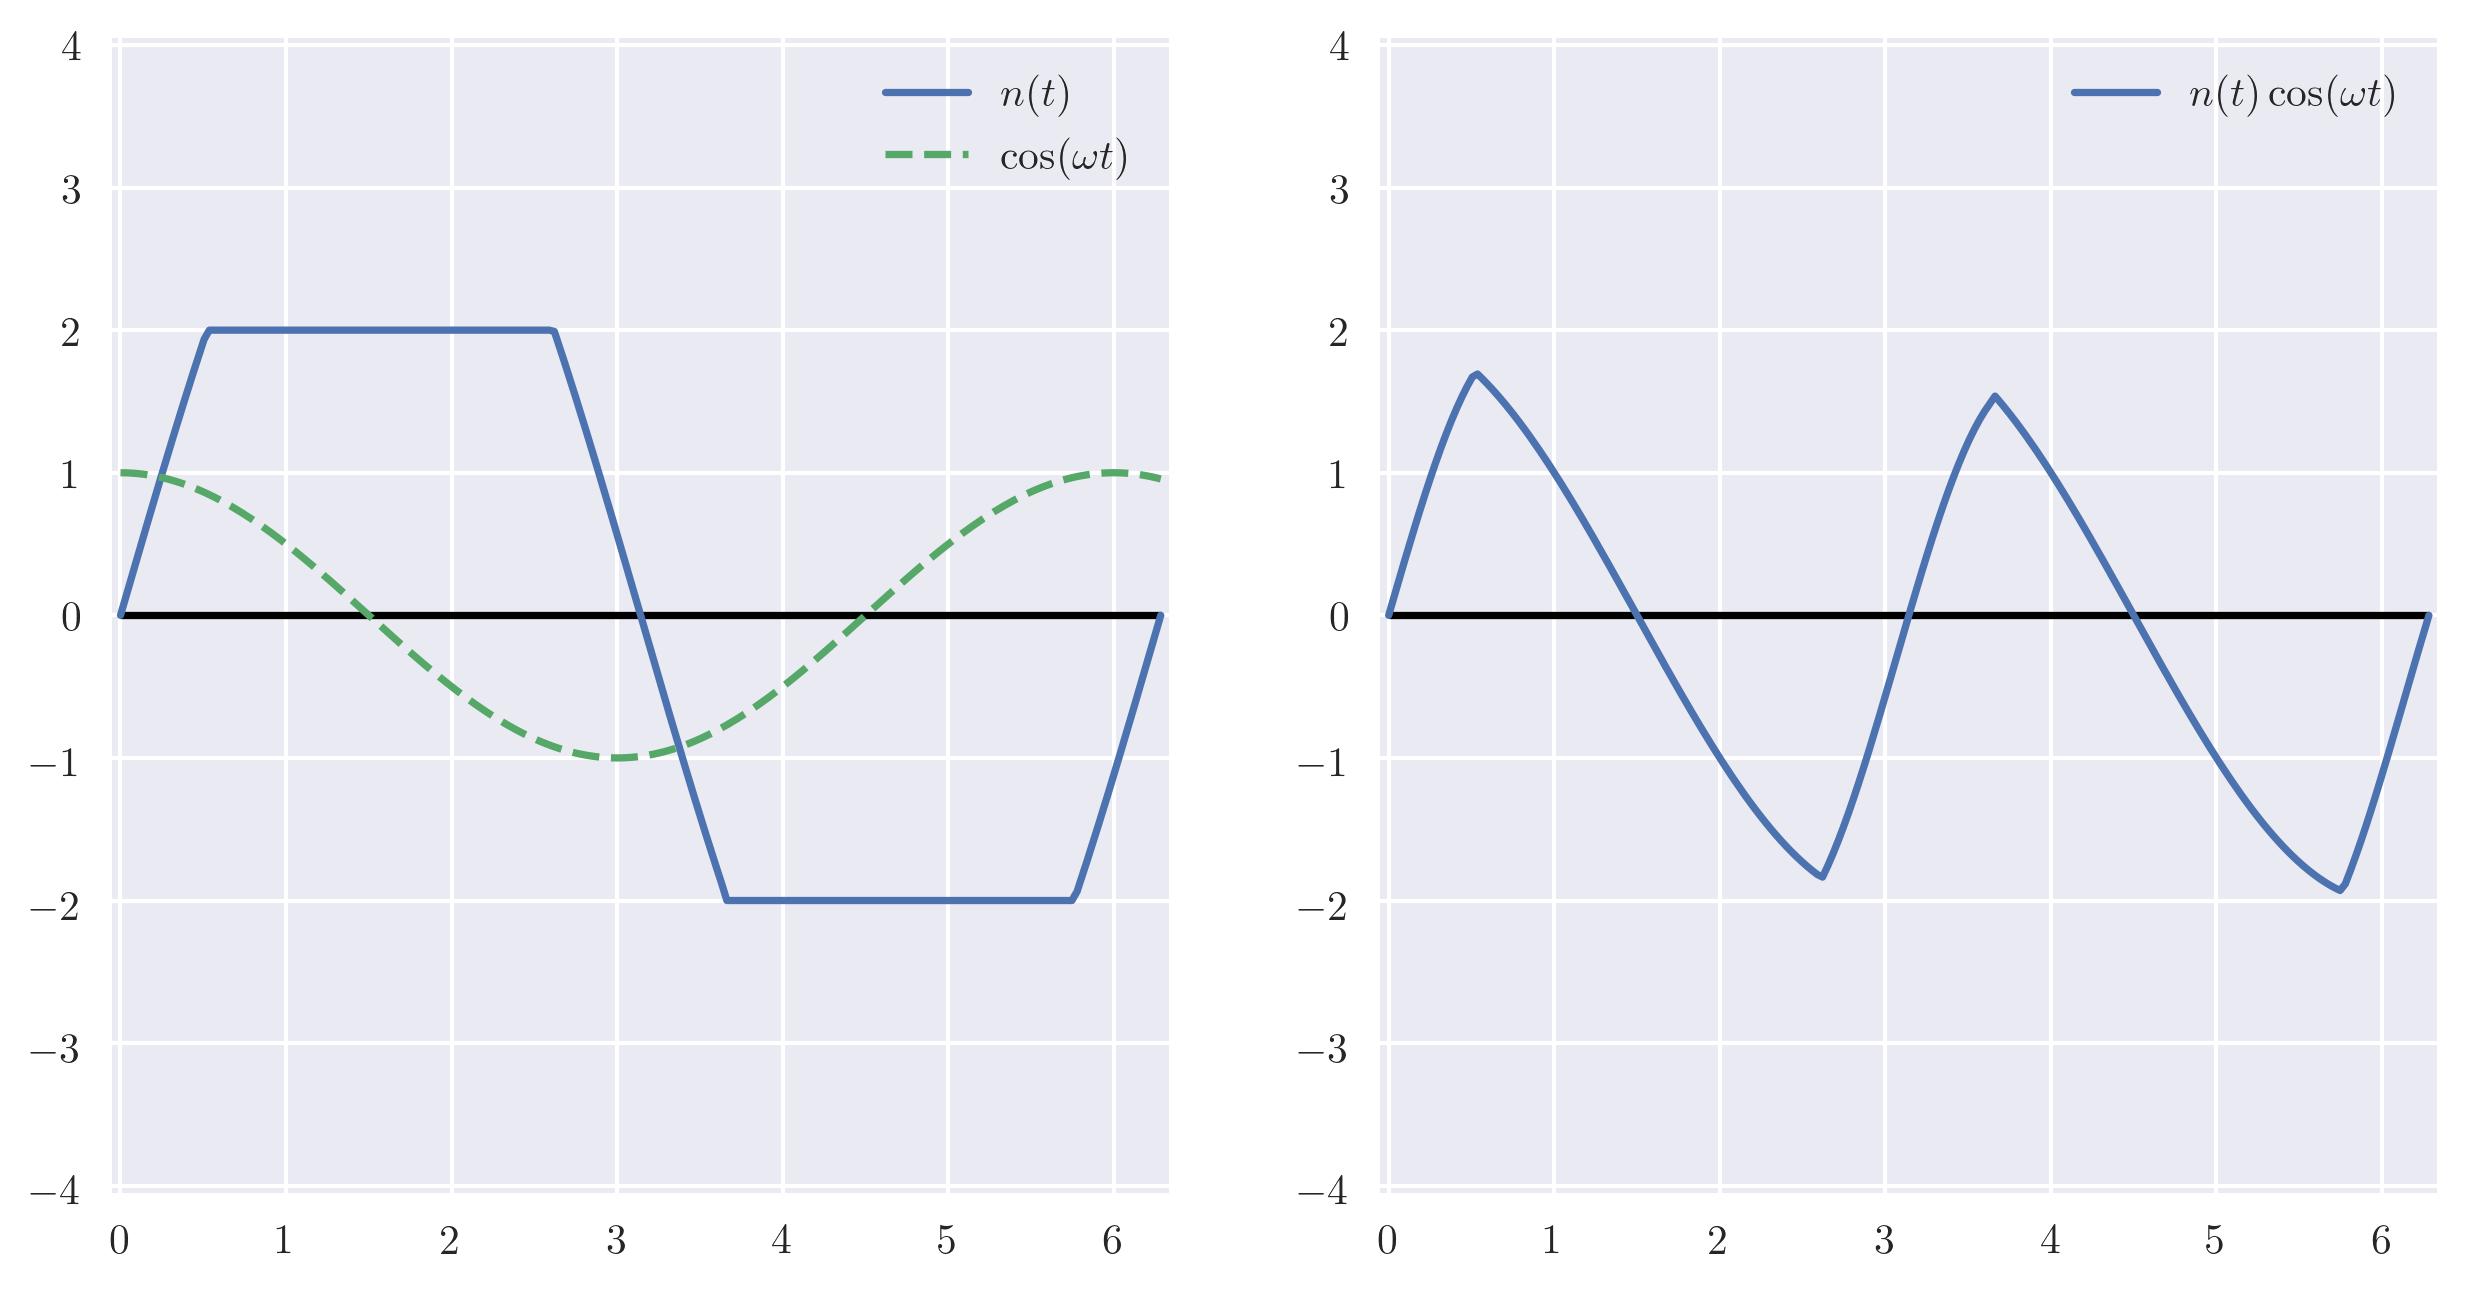
\includegraphics[width=\linewidth]{prod-ncos.png}
	\caption{Product of $n(t)$ and $\cos(\omega t)$, with $\abs{V} = 2$.}
	\label{fig:prod-ncos}
\end{figure}

Extending $n(t)$ in the negative direction shows that it is an odd function, and $\cos$ is an even function, so the resulting product is even. The integral of their product over one full period is zero. Thus, $A_1 = 0$. We apply the same graphical analysis to $B_1$ as in Fig. \ref{fig:prod-nsin}.

\begin{figure}[h!]
	\centering
	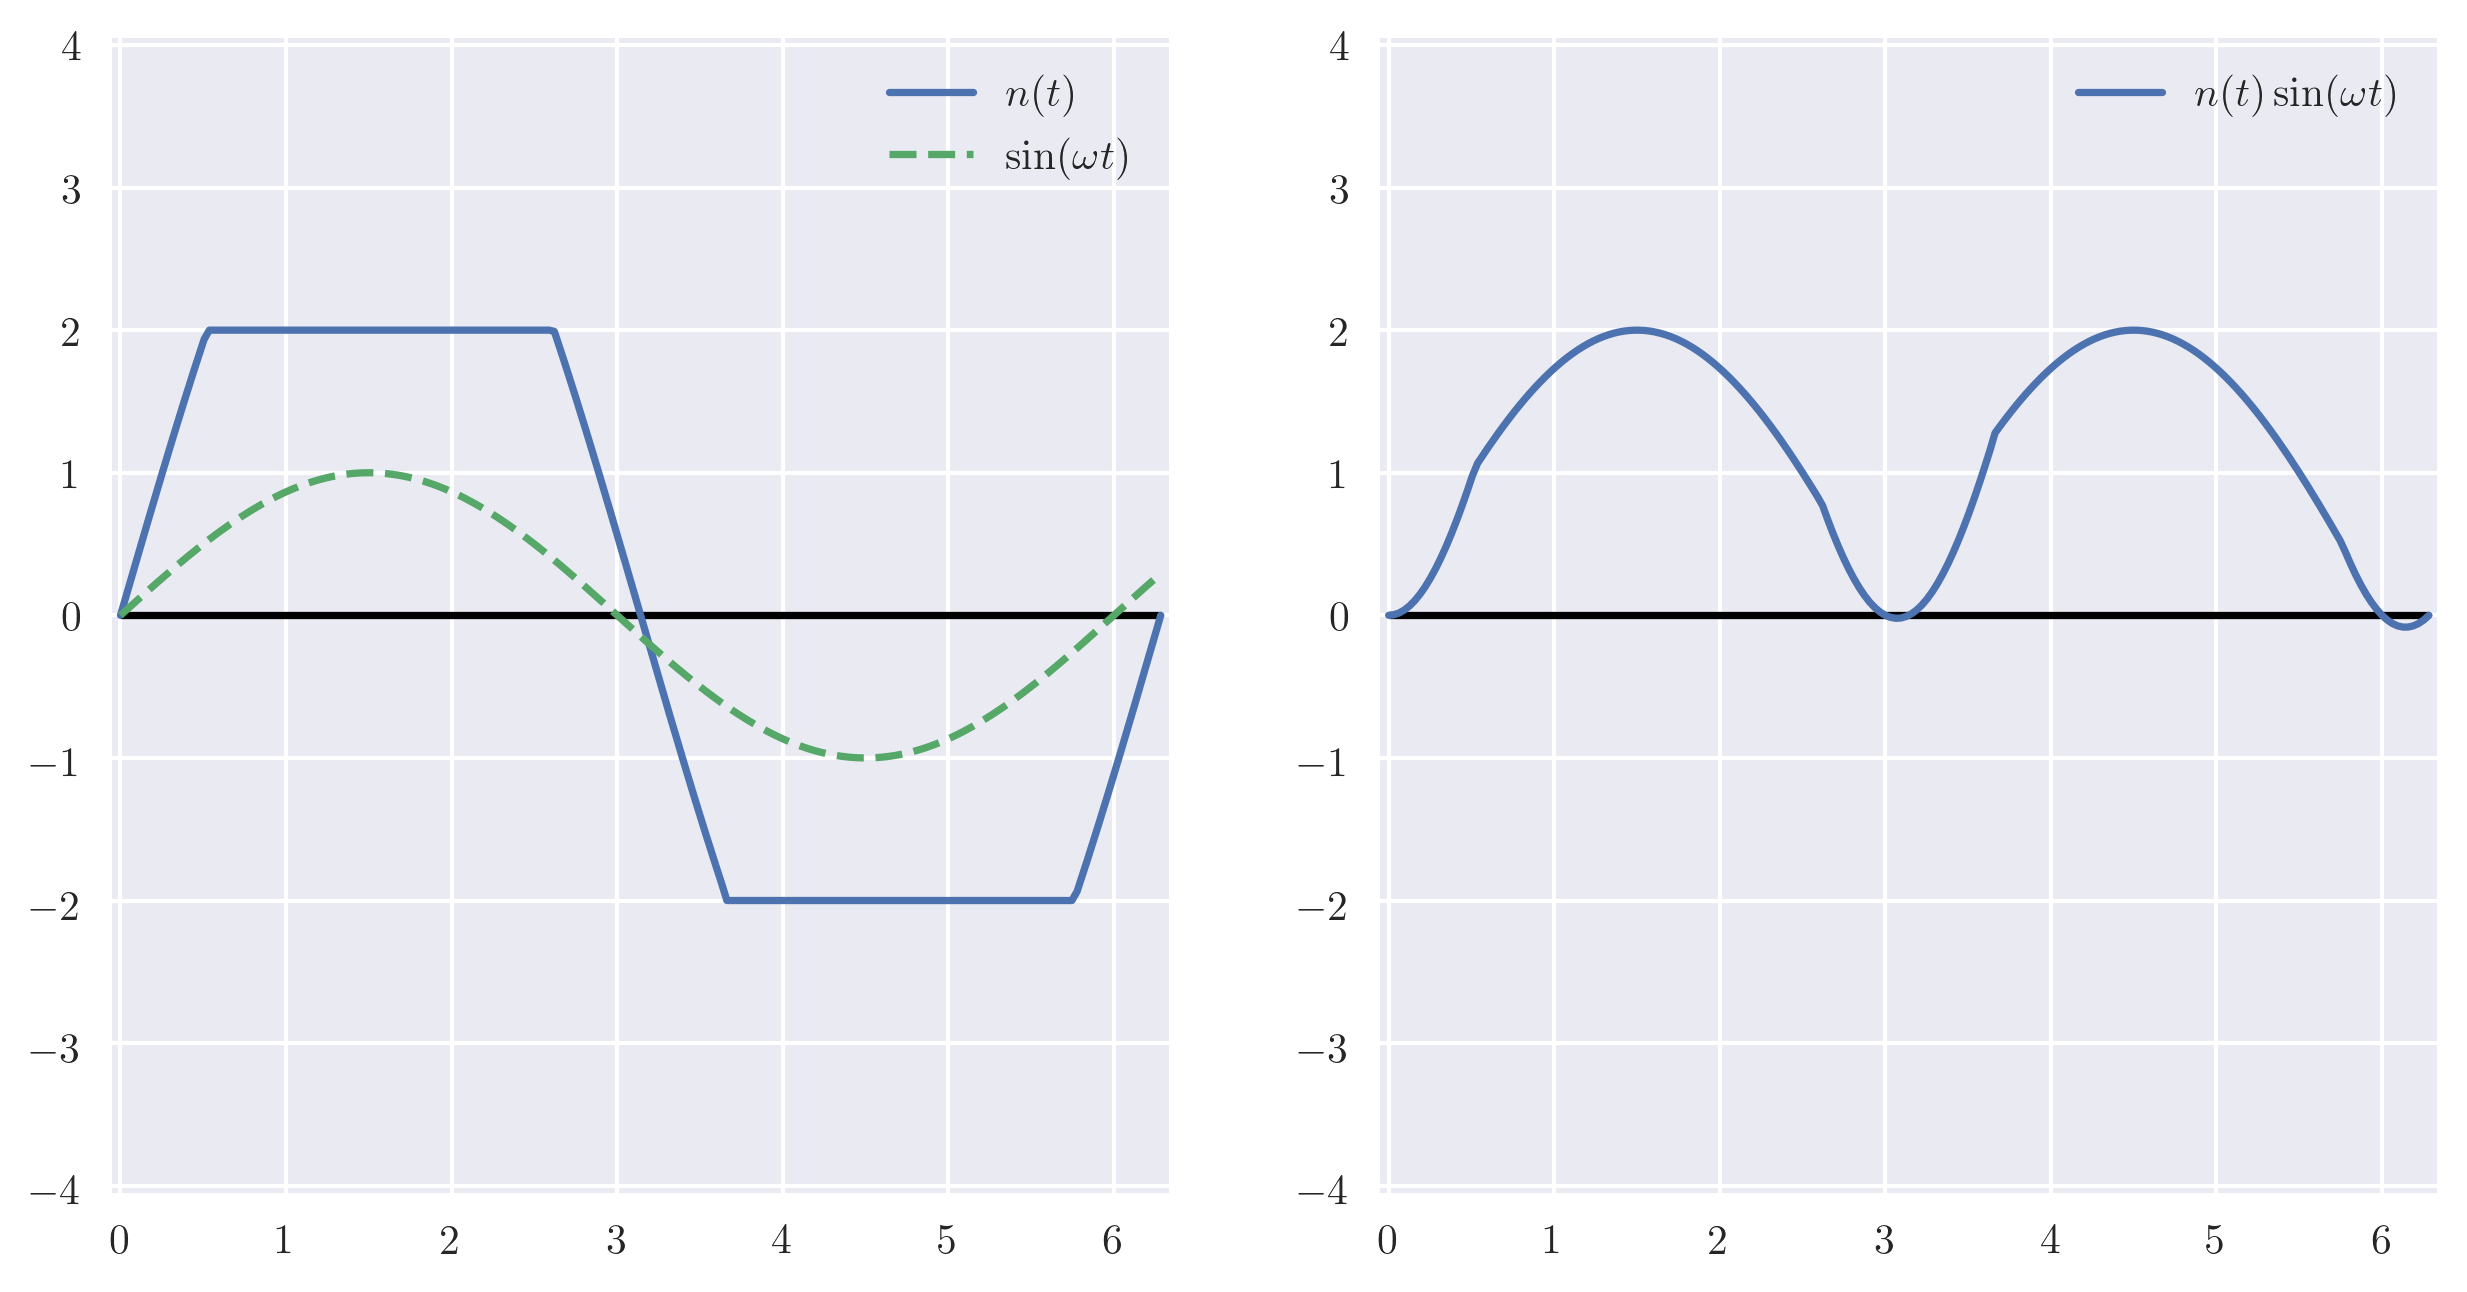
\includegraphics[width=\linewidth]{prod-nsin.png}
	\caption{Product of $n(t)$ and $\sin(\omega t)$, with $\abs{V} = 2$.}
	\label{fig:prod-nsin}
\end{figure}

In this case, $n(t)$ and $\sin(\omega t)$ are both odd functions, so the integral of their product is non-zero. We now have

\begin{equation}
	n(t) = B_1 \sin(\omega t)
\end{equation}

Solving for the coefficient $B_1$:

\begin{equation}
	B_1(t) = \frac{2}{T}\int_0^T n(t)\sin(\omega t)\dd{t}
\end{equation}

Notice that one wave period is made up of two symmetric patterns, both of which are in turn, symmetric about their respective centers. Thus, we need only to integrate $1/4$ of the area under the curve and multiply it by 4:

\begin{align}
	B_1(t) &= \frac{8}{T}\int_0^{T/4} n(t)\sin(\omega t)\dd{t} \\
	&= \frac{8}{T}\qty[\int_0^{\beta} kV\sin^2(\omega t)\dd{t} + \int_{\beta}^{\pi/2} ka\sin(\omega t)\dd{t}] \\
	&= \frac{8kV}{\omega T}\qty[\beta + \frac{a}{V}\sqrt{1 - \frac{a^2}{V^2}}]
\end{align}

Recall $T \equiv 2\pi/\omega$. We have,

\begin{equation}
	B_1(t) = \frac{4kV}{\pi}\qty[\beta + \frac{a}{V}\sqrt{1 - \frac{a^2}{V^2}}]
\end{equation}

Solving for $N(M, \omega)$:

\begin{align}
	N(M, \omega) &= \frac{B_1 + jA_1}{M} \\
	&= \frac{B_1}{M} \\
	\Aboxed{
		N(M, \omega) &= \frac{4kV}{M\pi}\qty[\beta + \frac{a}{V}\sqrt{1 - \frac{a^2}{V^2}}]
	}
\end{align}

\clearpage

\item \textbf{Dead Zone}

\begin{figure}[h!]
	\centering
	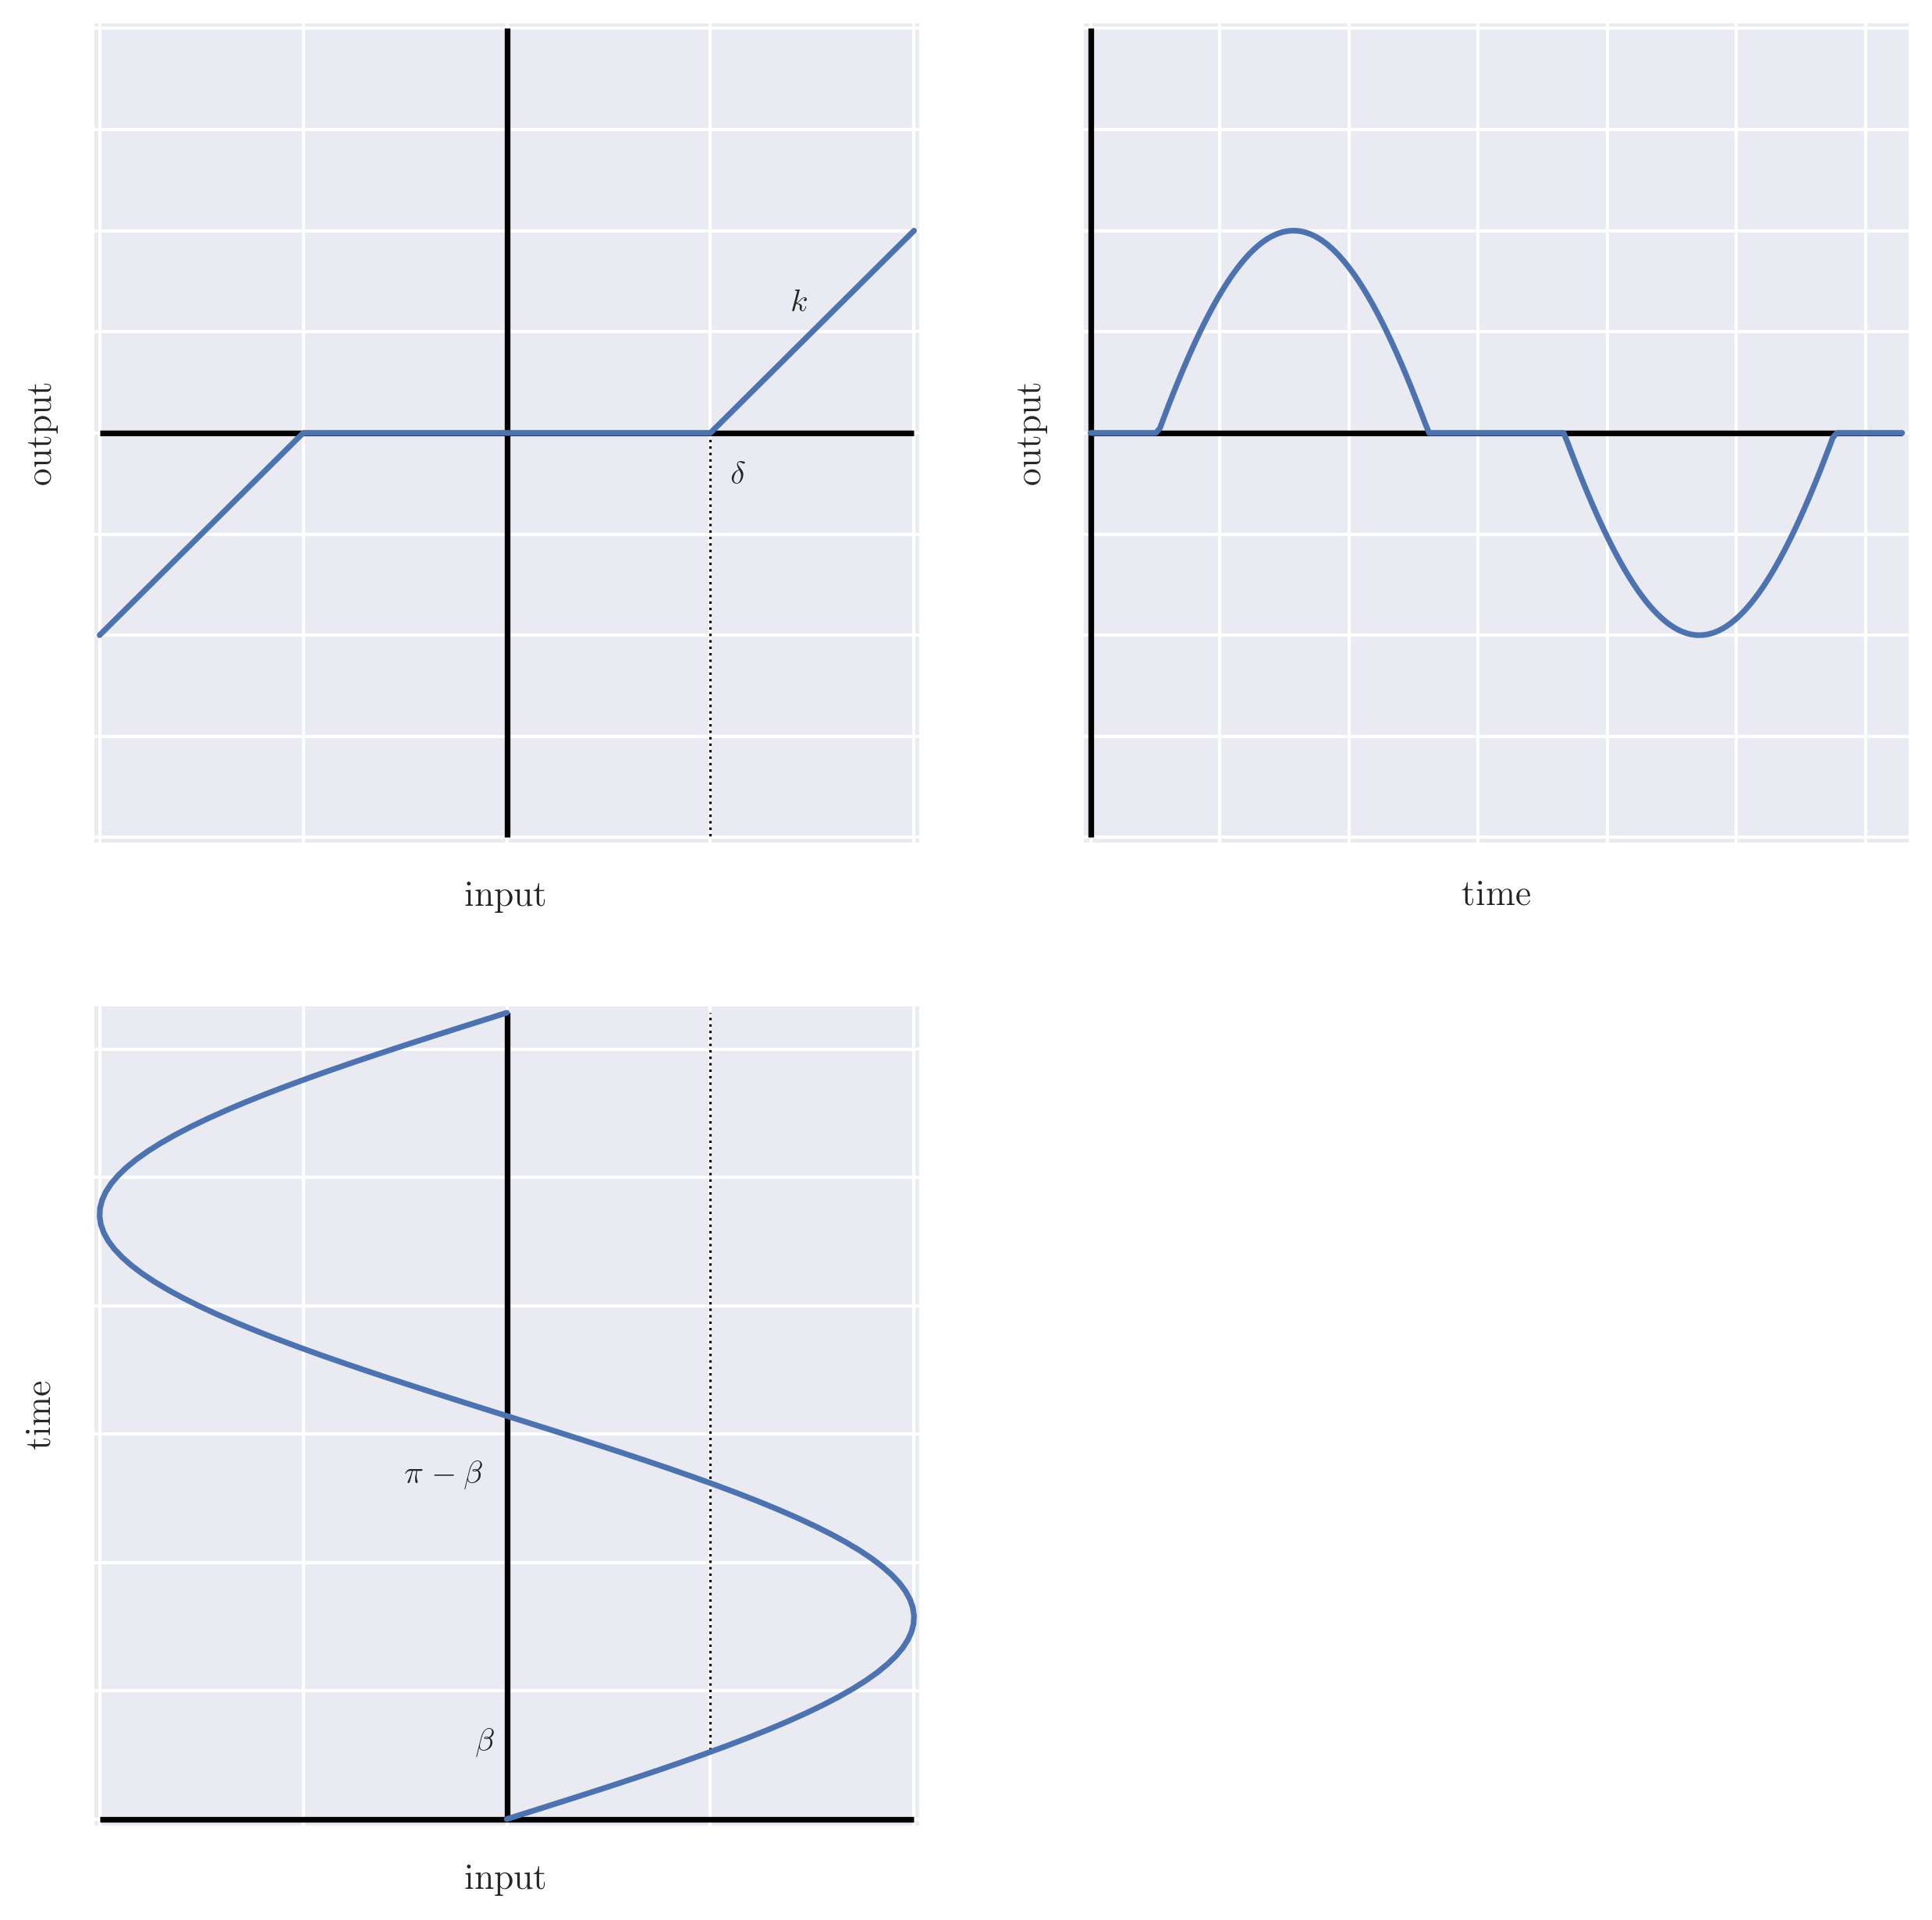
\includegraphics[width=\linewidth]{iocurve_dead.png}
	\caption{IO curves of a ramp with a dead zone and a sinusoidal input.}
	\label{fig:iocurve-dead}
\end{figure}

Consider again an input of the form $V\sin(\omega t)$. The output function is described by

\begin{equation}
	n(t) = 
	\begin{cases}
		0 \quad , & 0 \leq \omega t \leq \beta \\
		k[V\sin(\omega t) - \delta] \quad , & \beta \leq \omega t \leq \frac{\pi}{2}
	\end{cases}
\end{equation}

Following the same graphical analysis as before, we obtain Figs. \ref{fig:deadprod-ncos} and \ref{fig:deadprod-nsin}.

\begin{figure}[h!]
	\centering
	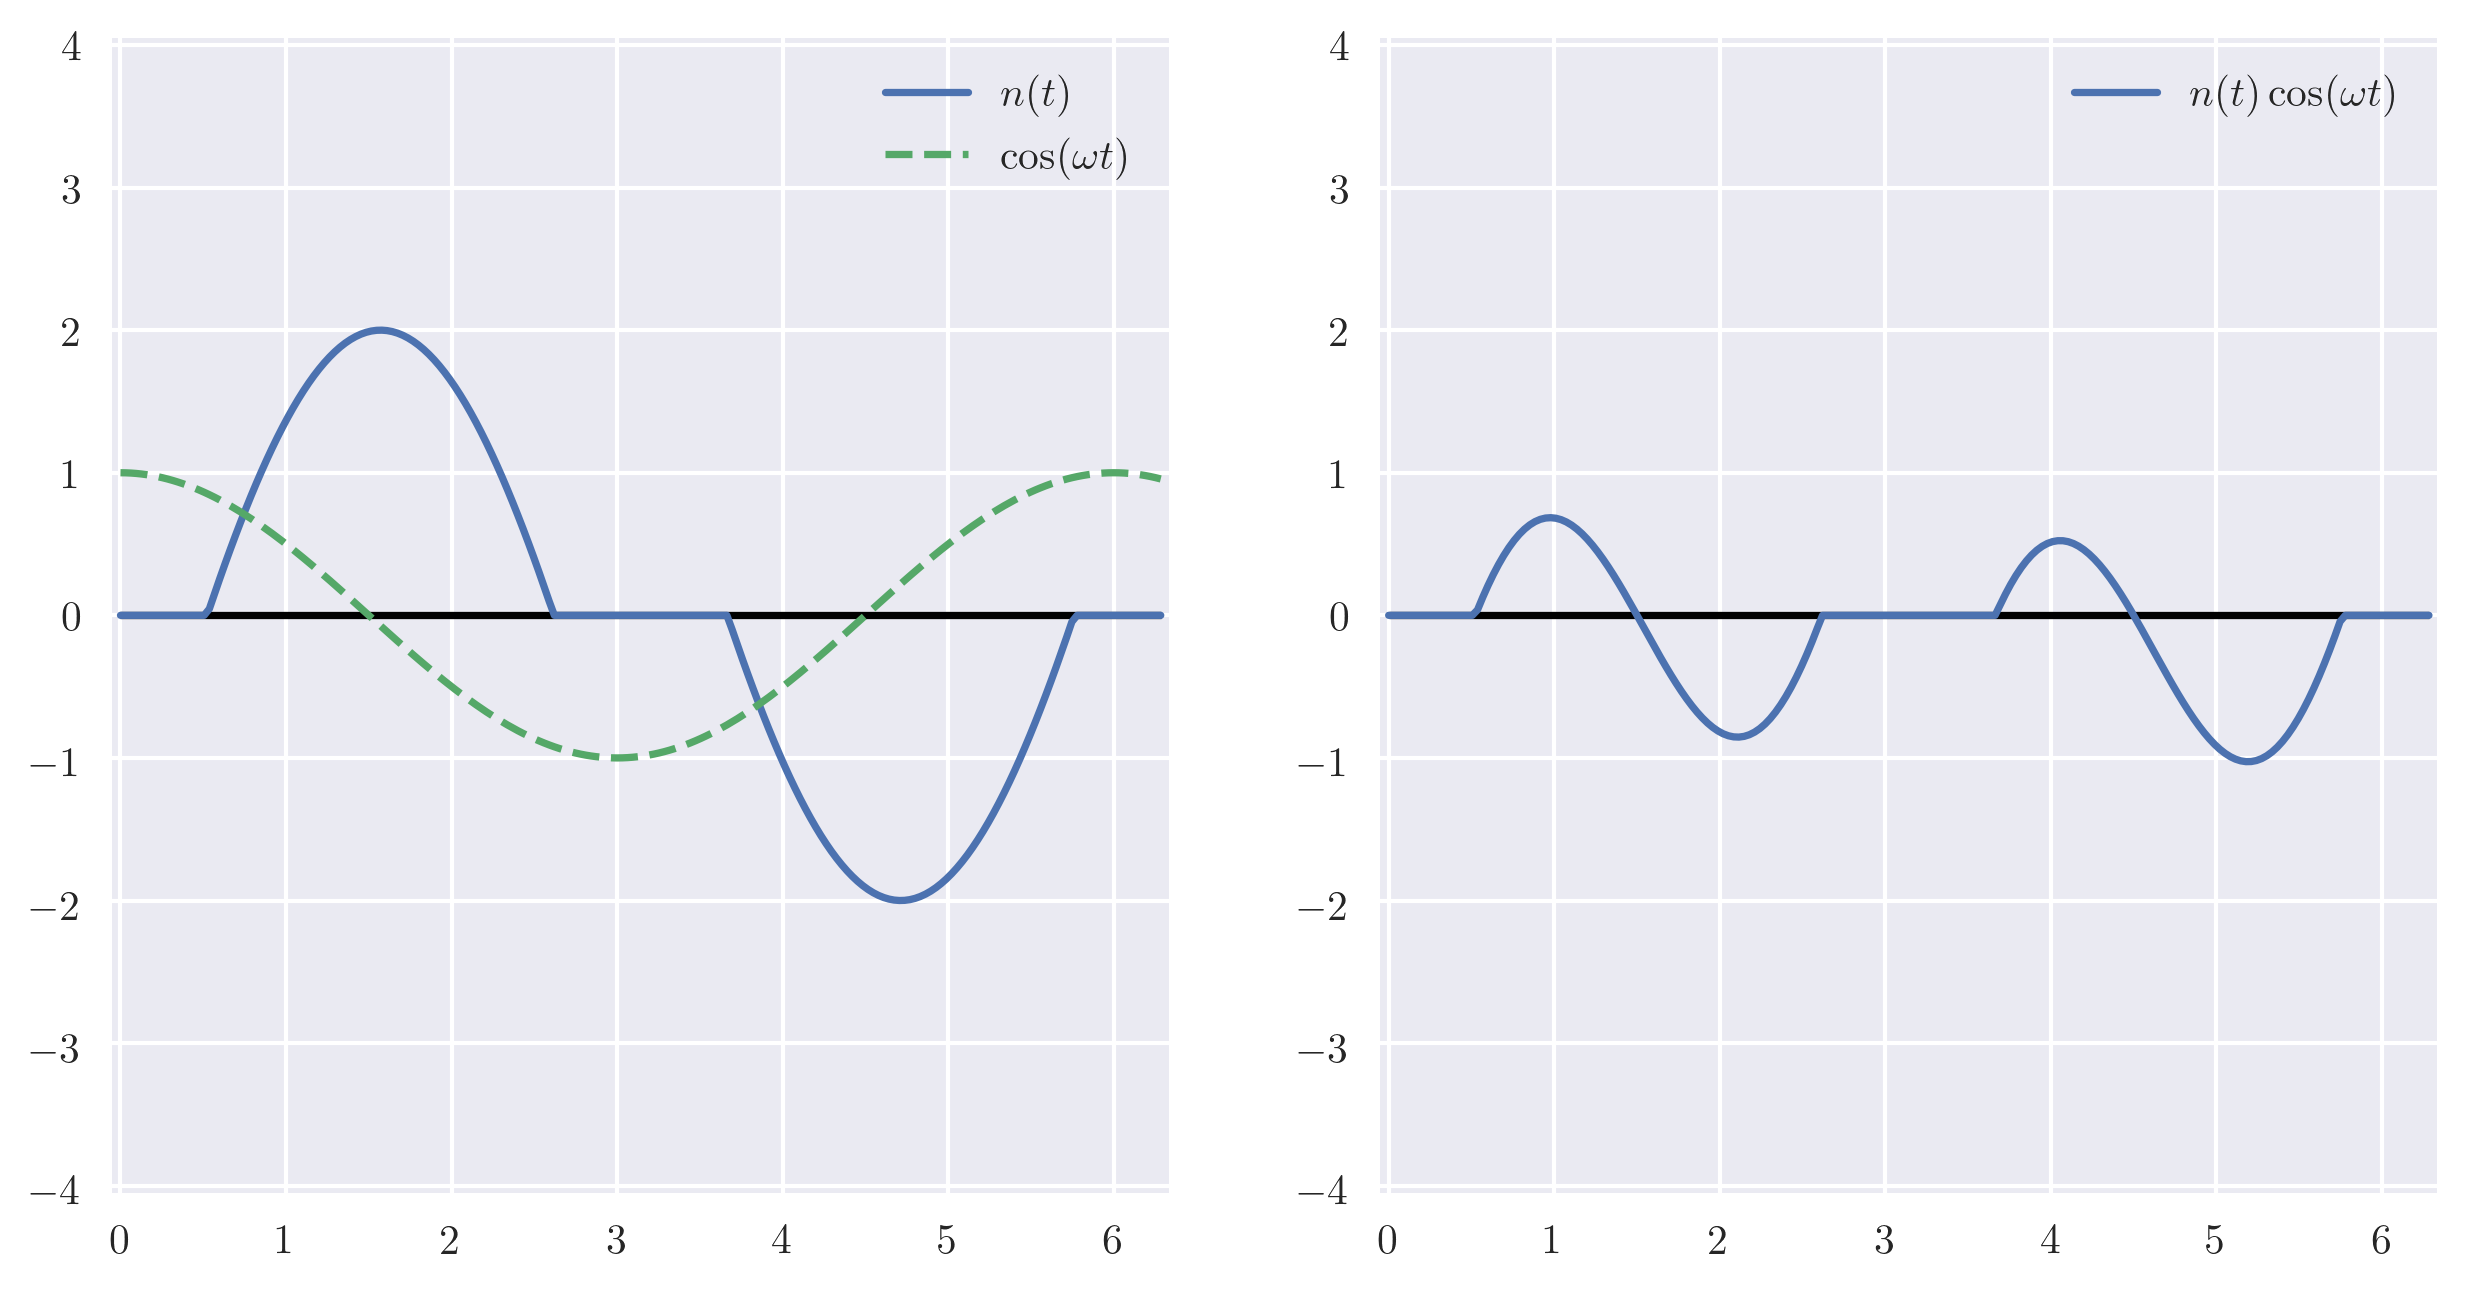
\includegraphics[width=\linewidth]{deadprod-ncos.png}
	\caption{Product of $n(t)$ and $\cos(\omega t)$, with $\abs{V} = 2$.}
	\label{fig:deadprod-ncos}
\end{figure}

\begin{figure}[h!]
	\centering
	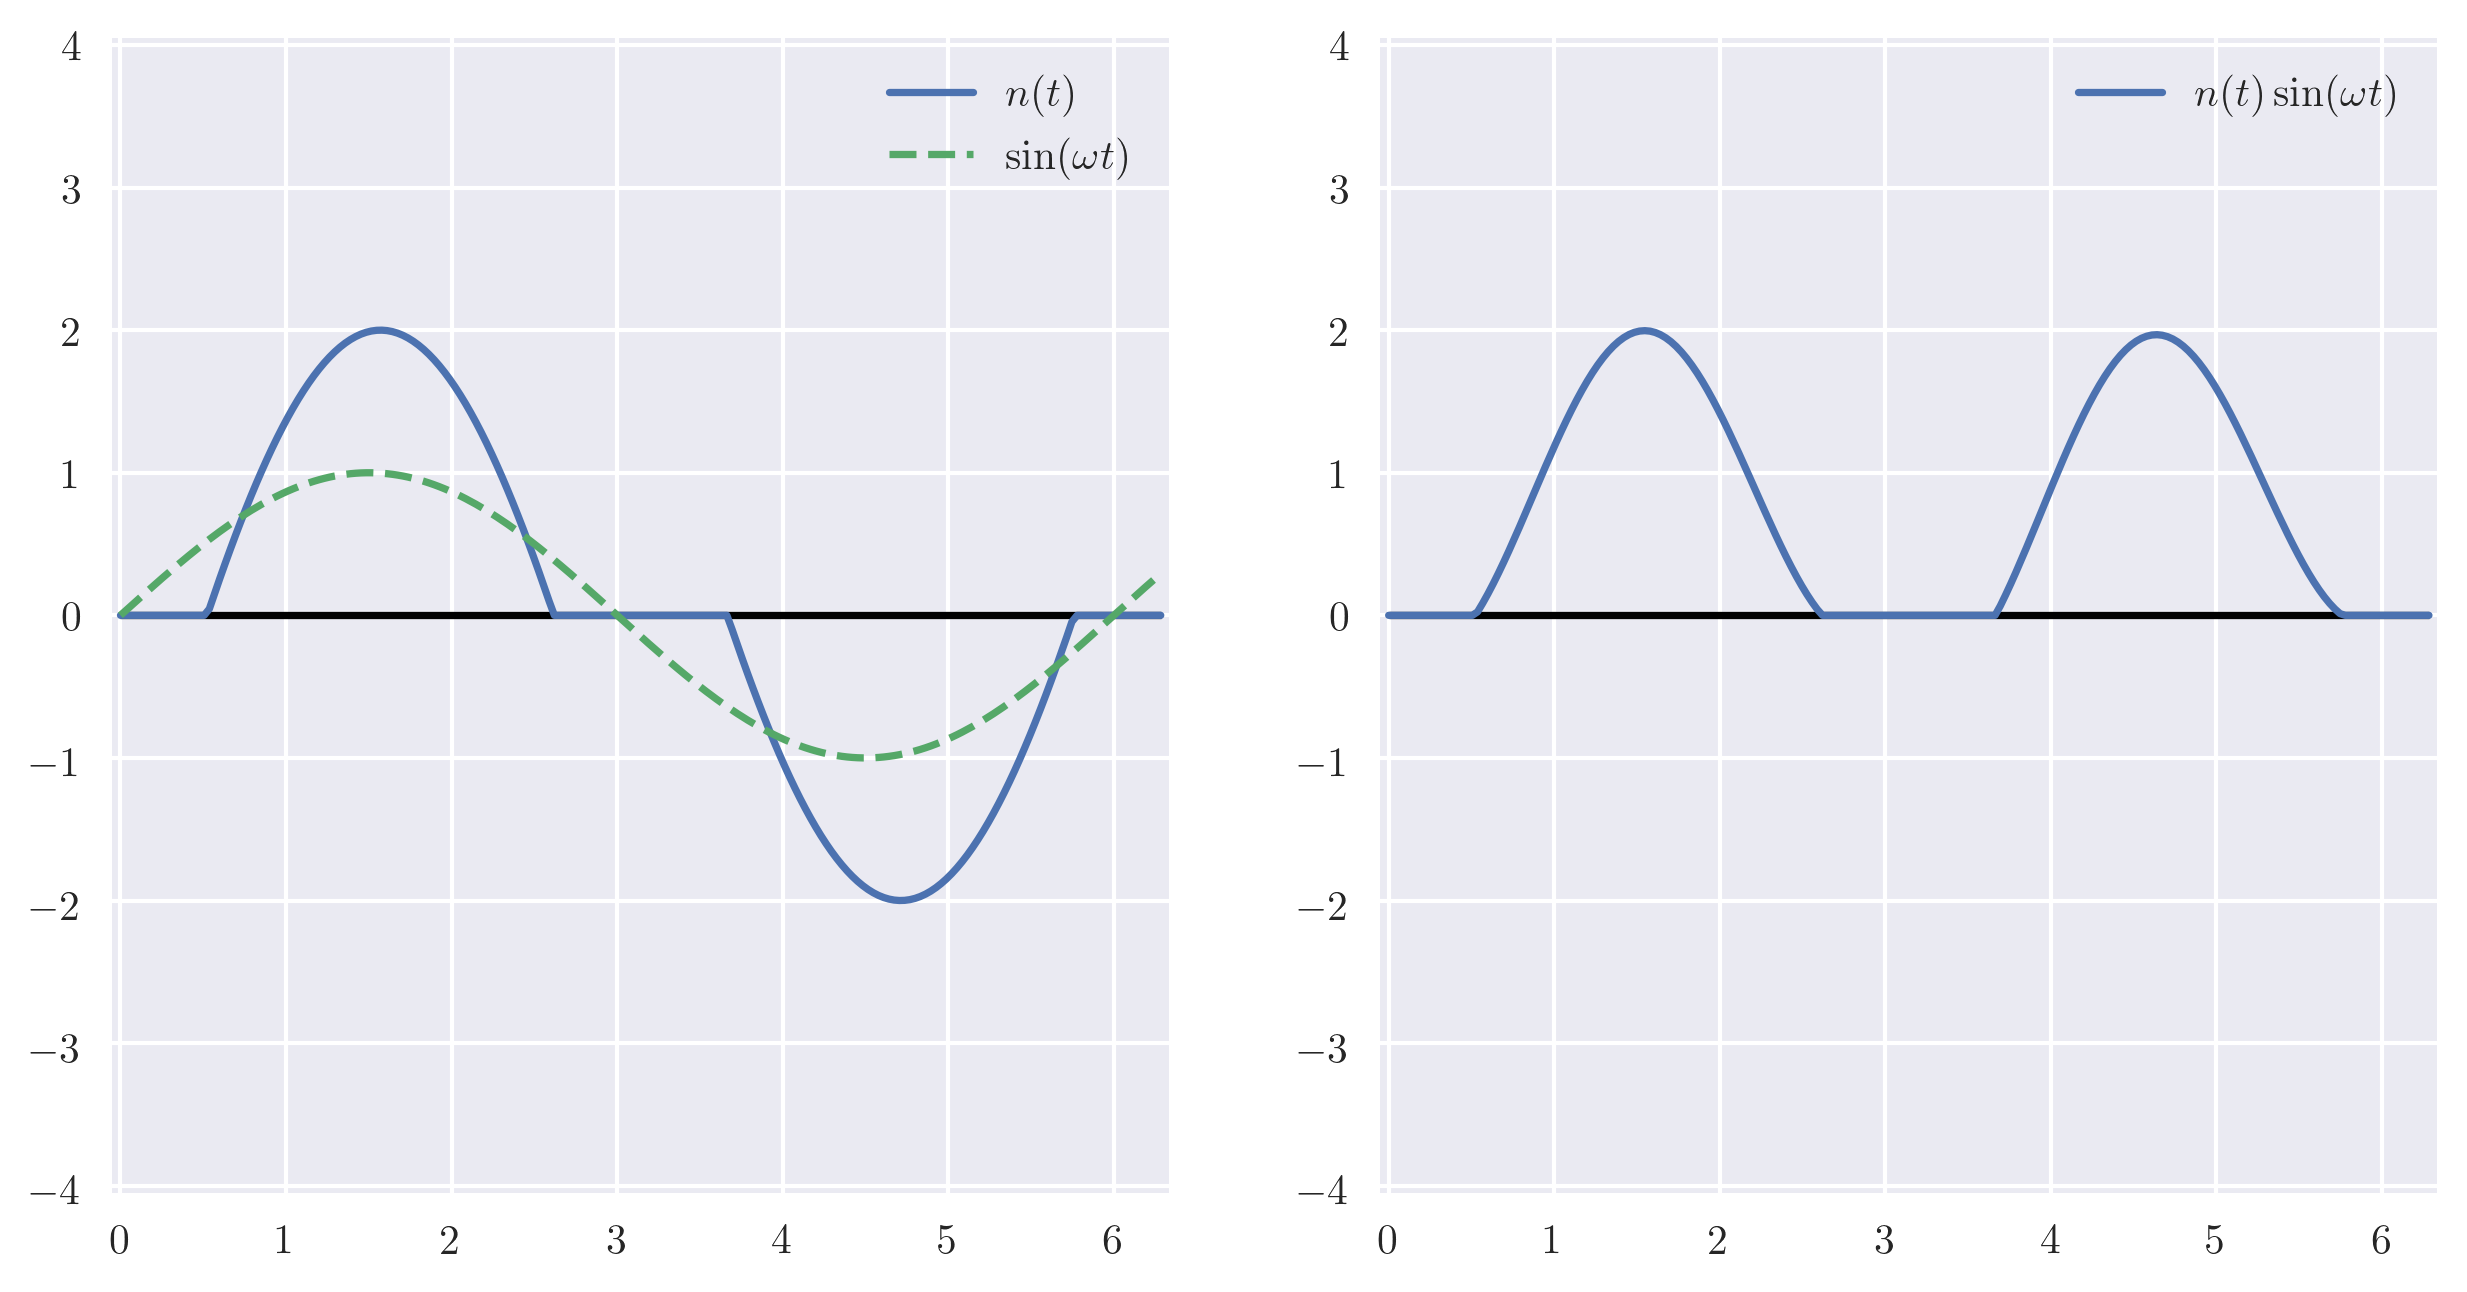
\includegraphics[width=\linewidth]{deadprod-nsin.png}
	\caption{Product of $n(t)$ and $\sin(\omega t)$, with $\abs{V} = 2$.}
	\label{fig:deadprod-nsin}
\end{figure}

We observe once again that the $\cos$ product is even, while the $\sin$ product is odd. Therefore, the $A_1$ term vanishes again and we are left to solve for $B_1$:

\begin{equation}
	B_1(t) = \frac{2}{T}\int_0^T n(t)\sin(\omega t) \dd{t}
\end{equation}

Following the same arguments as in the previous case,

\begin{align}
	B_1(t) &= \frac{8}{T}\int_0^{T/4} n(t)\sin(\omega t)\dd{t} \\
	&= \frac{8}{T}\qty[\int_\beta^{\pi/2} k\qty(V\sin(\omega t) - \delta)\sin(\omega t)\dd{t}] \\
	&= \frac{8V}{\omega T}\qty[\frac{\pi}{2} - \beta - \frac{\delta}{V}\sqrt{1 - \frac{\delta^2}{V^2}}]
\end{align}

By trigonometry, $\beta \equiv \arcsin(\delta/V)$, so that

\begin{align}
	B_1(t) &= \frac{8V}{\omega T}\qty[\frac{\pi}{2} - \arcsin(\frac{\delta}{V}) - \frac{\delta}{V}\sqrt{1 - \frac{\delta^2}{V^2}}] \\
	&= \frac{4V}{\pi}\qty[\frac{\pi}{2} - \arcsin(\frac{\delta}{V}) - \frac{\delta}{V}\sqrt{1 - \frac{\delta^2}{V^2}}] \\
	\Aboxed{
		N(M, \omega) &= \frac{4V}{\pi M}\qty[\frac{\pi}{2} - \arcsin(\frac{\delta}{V}) - \frac{\delta}{V}\sqrt{1 - \frac{\delta^2}{V^2}}]
	}
\end{align} 

\end{enumerate}

\end{document}